\section{Sequence Modeling: Recurrent and Recursive Nets}
\begin{multicols}{2}
	\subsection{Recurrent Nets}
	A recurrent neural network (\textbf{RNN}) is a neural network that is specialized for processing a sequence of values $\vx^{(1)},\dots,\vx^{(\tau)}$.
	They can scale to much longer sequences than would be practical for networks without sequence-based specialization.
	Most RNN can also process sequences of variable length.
	Just as for CNNs, a large part of the power comes from \textbf{parameter sharing}.
	If we had separate parameters for each value of the time index, we could not generalize to sequence lengths not seen during training.
	\begin{figure}[H]
		\centering
		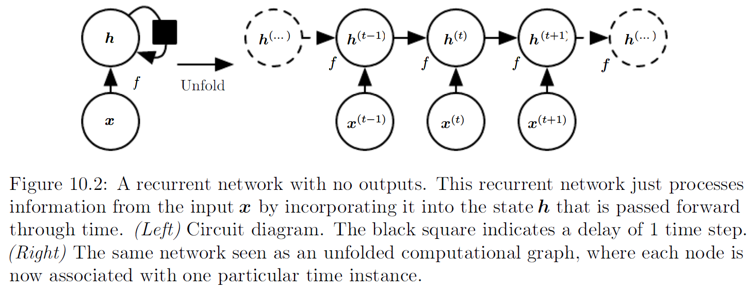
\includegraphics[width=\linewidth]{images/recurr1.png}
	\end{figure}
	
	RNNs share parameters in a different way than CNNs.
	Each member of the output is a function of the previous members of the output.
	Each member of the output is produced using the same update rule applied to the previous outputs.
	This recurrent formulation results in the sharing of parameters through a very deep computational graph.\\
	
	We refer to RNNs as operating on a sequence that contains vectors $\vx(t)$ with time step index $t$ ranging from 1 to $\tau$. 
	In practice, RNNs usually operate on minibatches of such sequences, with a different sequence length $\tau$ for each member of the minibatch.
	RNNs may also be applied in two dimensions across spatial data such as images, and even when applied to data involving time, the network may have connections that go backwards in time, provided that the entire sequence is observed before it is provided to the network.
	
	\subsection{Unfolding Computational Graphs}
	A computational graph is a way to formalize the structure of a set of computations, such as those involved in mapping inputs and parameters to outputs and loss.
	The idea of unfolding a recurrent computation into a computational graph that has a repetitive structure, typically corresponding to a chain of events.
	Unfolding this graph results in the sharing of parameters across a deep network structure.
	\begin{align*}
	\vs^{(t)} &= f\left(\vs^{(t-1)};\bolt\right)\\
	\vs^{(3)} &= f\left(\vs^{(2)};\bolt\right)\\
	&= f\left(f\left(\vs^{(1)};\bolt\right);\bolt\right)
	\end{align*}
	As another example, let us consider a dynamical system driven by an external signal $\vx^{(t)}$ with state $\vs^{(t)}$
	\[ \vs^{(t)} = f\left(\vs^{(t-1)},\vx^{(t)};\bolt\right) \]
	where we see that the state now contains information about the whole past sequence.\\
	
	To indicate that the state is the hidden units in the network, we now rewrite the equation using the variable $\vh$ to represent the (hidden) state:
	\[ \vh^{(t)} = f\left(\vh^{t-1},\vx^{(t)};\bolt\right) \]
	When the recurrent network is trained to perform a task that requires predicting the future from the past, the network typically learns to use $\vh^{(t)}$ as a kind of lossy summary of the task-relevant aspects of the past sequence of inputs up to $t$.
	This summary is in general necessarily lossy, since it maps an arbitrary length sequence $\vx^{(t)},\vx^{(t-1)},\dots,\vx^{(1)}$ to a fixed length vector $\vh^{(t)}$.\\
	
	We can represent the unfolded recurrence after $t$ steps with a function $g^{(t)}$. This function takes the whole past sequence as input and produces the current state.
	The unfolded recurrent structure allows us to factorize $g^{(t)}$ into repeated applications of a function $f$.
	\begin{align*}
	\vh^{(t)} &= g^{(t)}\left( \vx^{(t)},\vx^{(t-1)},\vx^{(t-2)},\dots,\vx^{(2)},\vx^{(1)} \right)\\
	&= f\left(\vh^{(t-1)},\vx^{(t)};\bolt\right)
	\end{align*}
	One major advantage of RNNs is, that it's possible to use the \textbf{same} transition function $f$ with the same parameters at every time step.
	Another one is, that regardless of the sequence length, the learned model always has the same input size, because it is specified in terms of transition from one state to another state, rather than specified in terms of a variable-length history of states.
	
	\subsection{Recurrent Neural Networks}
	There is a wide array of RNNs possible.\\
	RNNs that produce an output at each time step and have recurrent connections between hidden units:
	\begin{figure}[H]
		\centering
		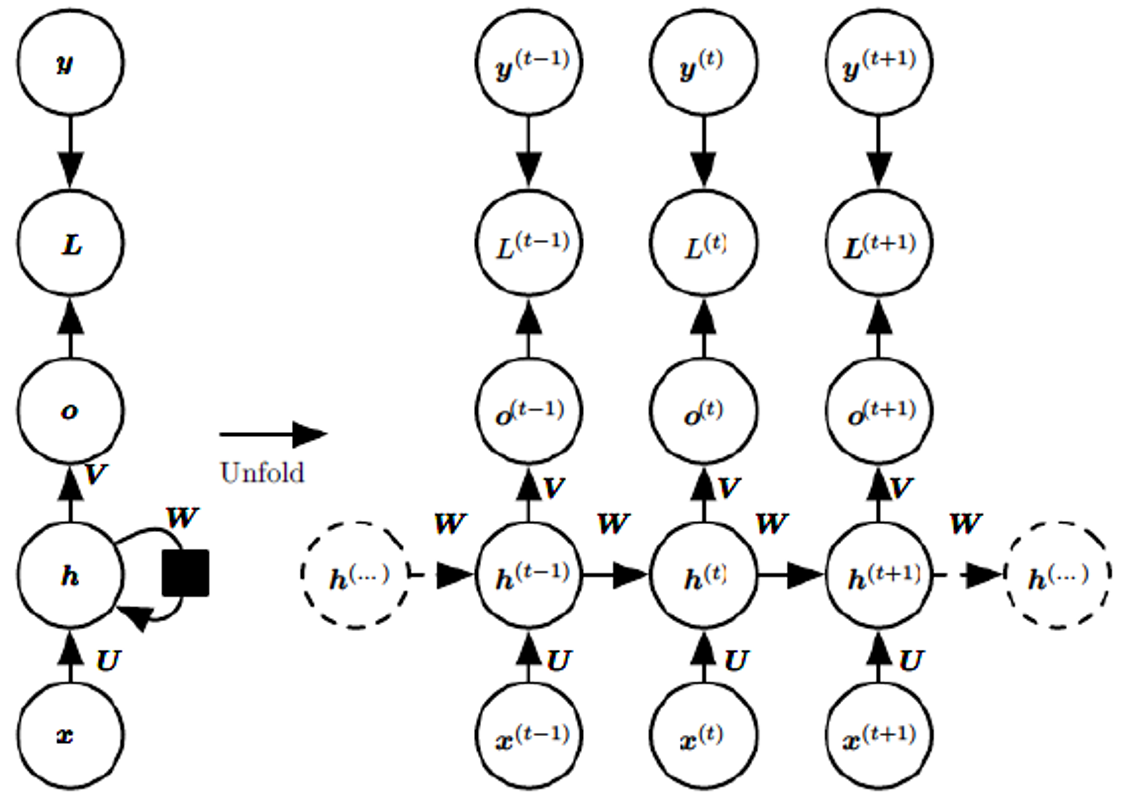
\includegraphics[width=0.8\linewidth]{images/rec1.PNG}
		\caption{This is the RNN we will refer to later}
	\end{figure}
	RNNs that produce an output at each time step and have recurrent connections only from the output at one time step to the hidden units at the next time step:
	\begin{figure}[H]
		\centering
		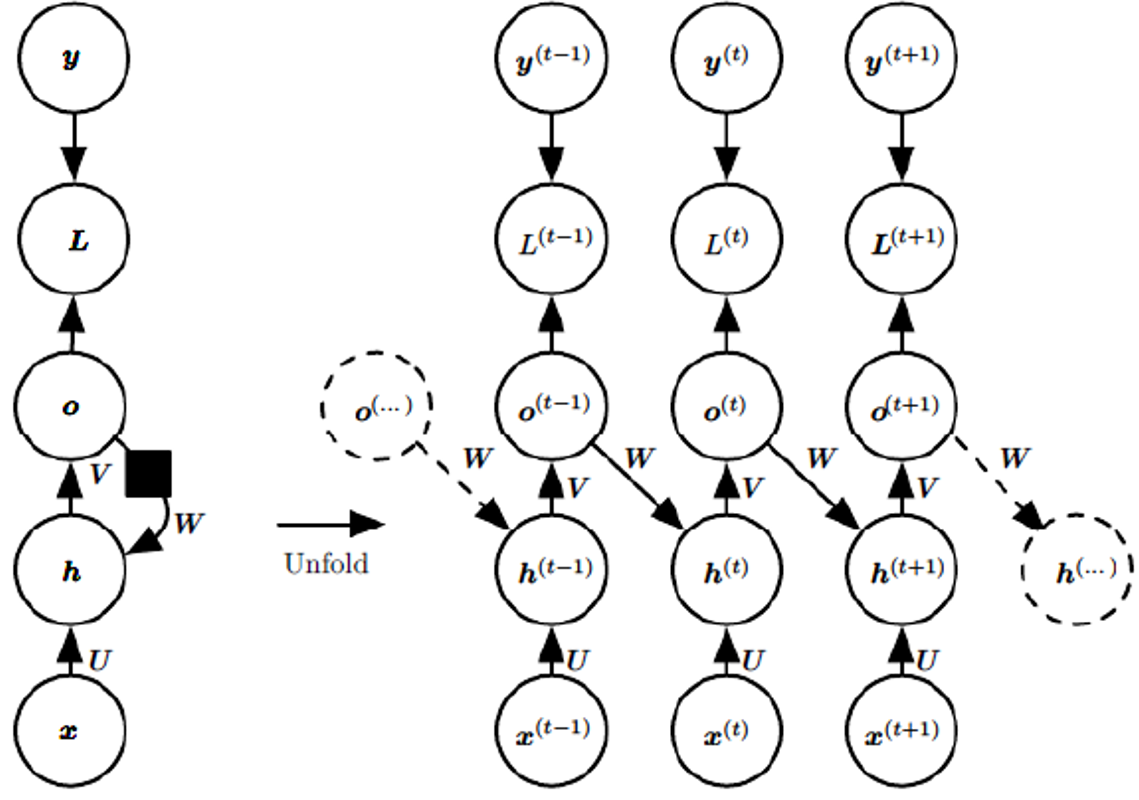
\includegraphics[width=0.8\linewidth]{images/rec2.PNG}
	\end{figure}
	RNNs with recurrent connections between hidden units, that read an entire sequence and then produce a single output:
	\begin{figure}[H]
		\centering
		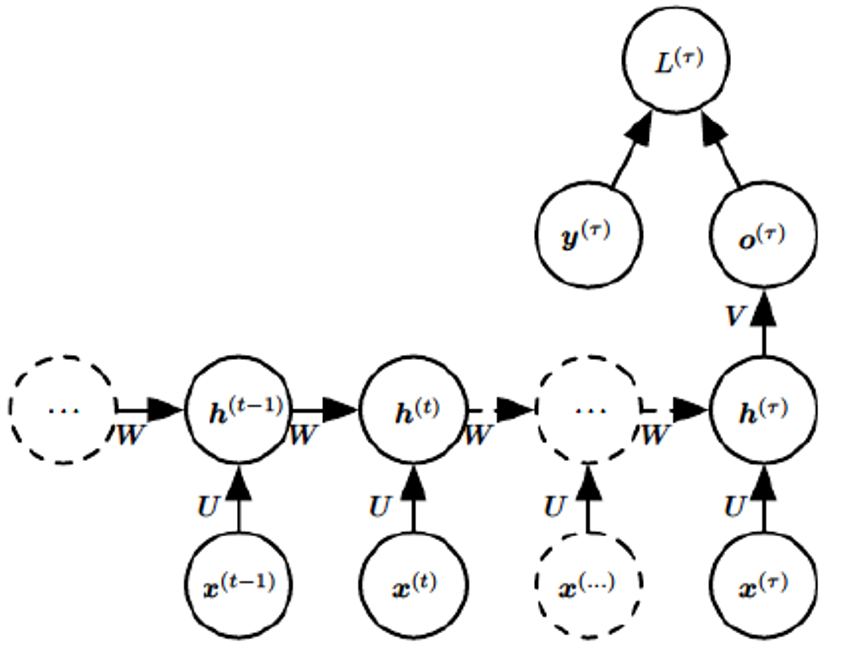
\includegraphics[width=0.7\linewidth]{images/rec3.PNG}
	\end{figure}
	
	\textbf{Forward propagation} begins with a specification of the initial state $\vh^{(0)}$.
	Then, for each time step from $t=1$ to $t=\tau$, we apply the update equations
	\begin{align*}
	\va^{(t)} &= \vb+\mW\vh^{(t-1)} +\mU\vx^{(t)}\\
	\vh^{(t)} &= \tanh(\va^{(t)})\\
	\vo^{(t)} &= \vc+\mV\vh^{(t)}\\
	\hat{\vy}^{(t)} &= \softmax(\vo^{(t)})
	\end{align*}
	where the parameters are the bias vectors $\vb$ and $\vc$, along with the weight matrices $\mU$, $\mV$ and $\mW$, respectively for input-to-hidden, hidden-to-output and hidden-to-hidden connections.\\
	
	In figure 1 is an example of a RNN that maps an input sequence to an output sequence of the same length.
	The total loss for a given sequence of $\vx$ values paired with a sequence of $\vy$ values would then be just the sum of the losses over all the time steps.
	For example, if $L^{(t)}$ is the negative log-likelihood of $y^{(t)}$, given $\vx^{(1)},\dots,\vx^{(t)}$, then the loss function is calculated as
	\begin{align*}
	& L\left( \{ \vx^{(1)},\dots,\vx^{(\tau)} \}, \{ \vy^{(1)},\dots,\vy^{(\tau)} \} \right)\\
	&= \sum_t L^{(t)}\\
	&= -\sum_t \log p_{\text{model}}\left(y^{(t)}| \{ \vx^{(1)},\dots,\vx^{(t)} \} \right)
	\end{align*}
	$y^{(t)}$ is the current discrete desired output element (for example a word).
	The output of the softmax is a vector containing the estimated probabilities for each possible discrete output element (for example a word or a character).\\
	
	Computing the gradient for a typical RNN of this loss function with respect to the parameters is an expensive operation.
	The gradient computation involves performing a forward propagation pass moving left to right through the figure 1, followed by a backward propagation pass moving right to left through the graph.
	The runtime is $O(\tau)$ and cannot be reduced by parallelization because the forward propagation is inherently sequential; each time step may only be computed after the previous one.
	States computed in the forward pass must be stored until they are reused during the backward pass, so the memory cost is also $O(\tau)$.\\
	
	Gradient might explode, when the RNN is computed over many time steps.
	To avoid this, the update must be chosen to be small enough to avoid traversing too much upward curvature.
	We typically use learning rates that decay slowly enough that consecutive steps have approximately the same learning rate.
	A step size that is appropriate for a relatively linear part of the landscape is often inappropriate and causes uphill motion if we enter a more curved part of the landscape on the next step.
	\begin{figure}[H]
		\centering
		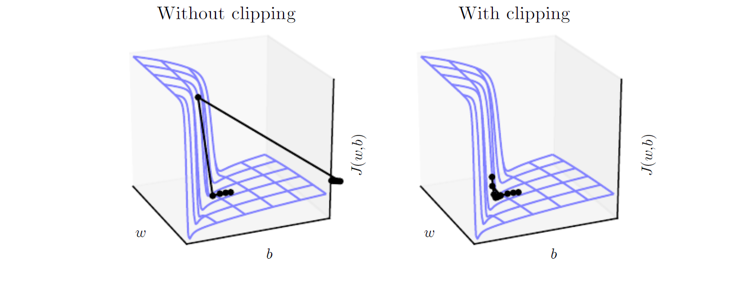
\includegraphics[width=0.9\linewidth]{images/clipping.png}
	\end{figure}
	One option is to \textbf{clip} the parameter gradient from a minibatch element-wise just before the parameter update.
	Another is to clip the norm of the gradient just before the parameter update:
	\[ \text{if } \lVert\vg\rVert > v \qquad\rightarrow\qquad \vg \leftarrow\frac{\vg v}{\lVert\vg\rVert} \]
	Although the parameter update has the same direction as the true gradient, with gradient norm clipping, the parameter update vector norm is now bounded.
	
	\subsection{Bidirectional RNNs}
	In many applications we want to output a prediction of $y^{(t)}$ which may depend on the \textbf{whole input sequence}.
	For example, in speech recognition, the correct interpretation of the current sound as a phoneme may depend on the next few phonemes because of co-articulation.
	Bidirectional RNNs combine an RNN that moves forward through time beginning from the start of the sequence with another RNN that moves backward through time beginning from the end of the sequence.
	\begin{figure}[H]
		\centering
		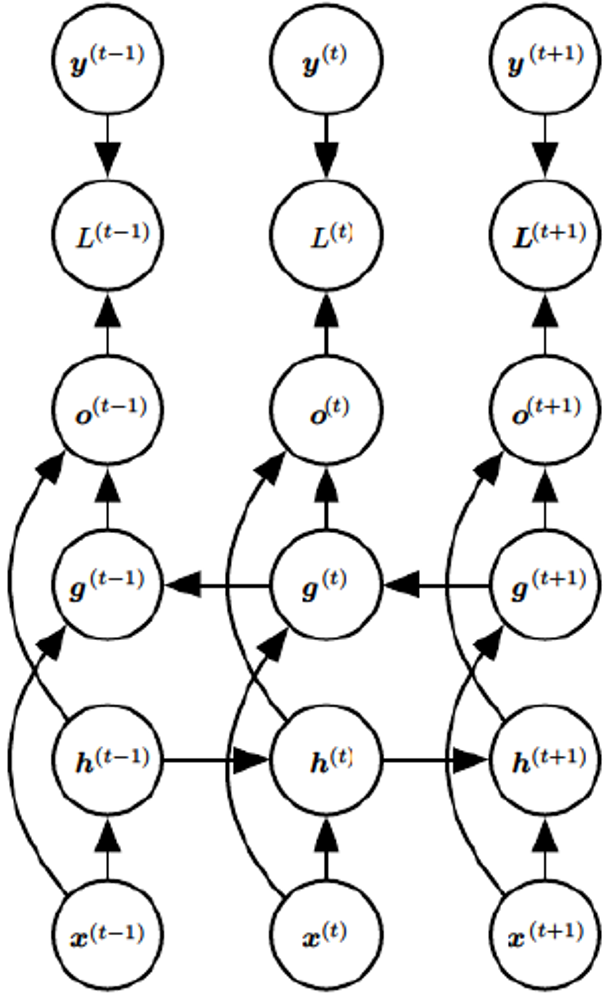
\includegraphics[width=0.4\linewidth]{images/bidir.PNG}
	\end{figure}
	The figure above illustrates the typical bidirectional RNN, with $\vh^{(t)}$ standing for the state of the sub-RNN that moves forward through time and $\vg^{(t)}$ standing for the state of the sub-RNN that moves backward through time.
	This allows the output units $\vo^{(t)}$ to compute a representation that depends on both the past and the future but is most sensitive to the input values around time $t$, without having to specify a fixed-size window around $t$.\\
	
	This idea can be naturally extended to a 2D input, such as images, by having four RNNs, each one going in one of the four directions.
	At each point $(i,j)$ of a 2D grid, an output could then compute a representation that would capture mostly local information but could also depend on long-range inputs.
	Compared to a CNN, RNNs applied to images are typically more expensive but allow for long-range lateral interactions between features in the same feature map.
	
	\subsection{Encoder-Decoder Sequence-to-Sequence Architectures}
	Mapping input sequences to output sequences of different lengths.
	We often call the input to the RNN the \textbf{context}. We want to produce a representation of this context, $\mC$. The context $\mC$ might be a vector or sequence of vectors that summarize the input sequence.\\
	In a sequence-to-sequence architecture, the two RNNs are trained jointly to maximize the average of the log conditional probability on the right over all the pairs of $\vx$ and $\vy$ sequences in the training set.
	\[ \log P(\vy^{(1)},\dots,\vy^{(n_y)}|\vx^{(1)},\dots,\vx^{(n_x)}) \]
	\begin{figure}[H]
		\centering
		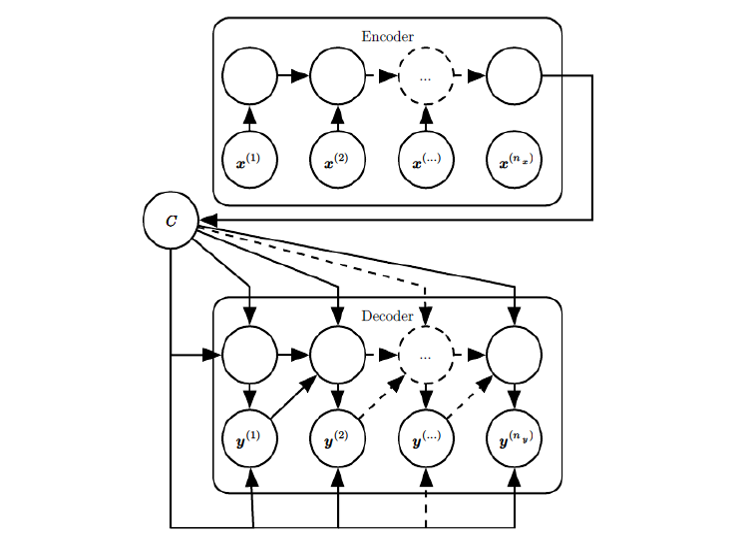
\includegraphics[width=0.8\linewidth]{images/encdec.png}
	\end{figure}
	The last state $\vh^{(n_x)}$ of the encoder RNN is typically used as a representation $\mC$ of the input sequence that is provided as input to the decoder RNN.
	One clear \textbf{limitation} of this architecture is when the context $\mC$ output by the encoder RNN has a dimension that is too small to properly summarize a long sequence.
	
	\subsection{Deep Recurrent Networks}
	The computation in most RNNs can be decomposed into three blocks of parameters and associated transformations\dots
	\begin{itemize}
		\item[\dots] from the input to the hidden state
		\item[\dots] from the previous hidden state to the next hidden state
		\item[\dots] from the hidden state to the output
	\end{itemize}
	
	\textbf{Introducing depth} can be done by many ways:
	\begin{figure}[H]
		\centering
		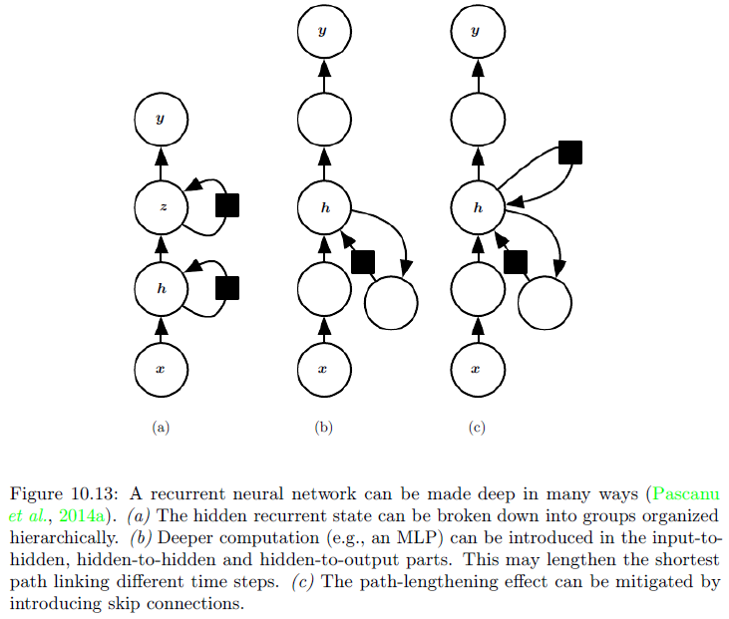
\includegraphics[width=0.9\linewidth]{images/rnn.png}
	\end{figure}
	
	\subsection{The Challenge of Long-Term Dependencies}
	The basic problem is that gradients propagated over many stages tend to either vanish or explode.
	Even if we assume that the parameters are such that the RNN is stable (can store memories, gradients not exploding), the difficulty with long-term dependencies arises from the exponentially smaller weights given to long-term interactions (involving the multiplication of many Jacobians) compared to short-term ones.\\
	RNN involve the composition of the same function multiple times, once per time step.
	These compositions can result in extremely nonlinear behavior, as illustrated in the figure below.
	\begin{figure}[H]
		\centering
		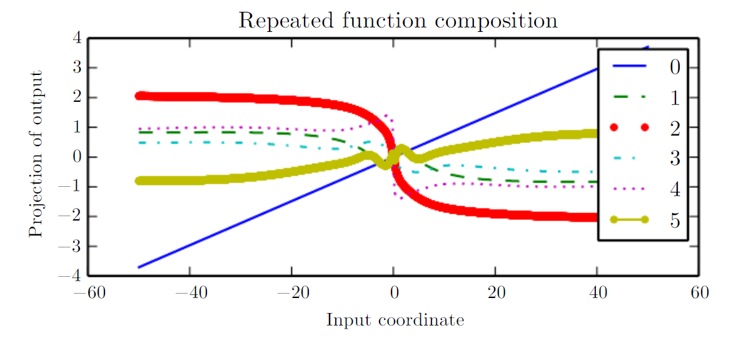
\includegraphics[width=0.9\linewidth]{images/unstable.png}
	\end{figure}
	The function composition employed by RNNs somewhat resembles matrix multiplication.
	We can think of the recurrence relationship on the right, as a simple RNN lacking a nonlinear activation function and lacking inputs:
	\[ \vh^{(t)} = \mW^T\vh^{(t-1)} \]
	This relationship can be simplified to
	\[ \vh^{(t)} = (\mW^t)^T \vh^{(0)} \]
	The eigenvalues are raised to the power of $t$ causing eigenvalues with magnitude less than one to decay to zero, and eigenvalues with magnitude greater than one to explode.
	Any component of $\vh^{(0)}$ that is not aligned with the largest eigenvector will eventually be discarded.\\
	
	If we make a non-recurrent network that has a different weight $w^{(t)}$ at each time step, and the initial state is given by 1, then the state at time $n$ is given by
	\[ \prod_{t=1}^{n}w^{(t)} \]
	
	Suppose that the $w^{(t)}$ values are generated randomly independently from one another, with zero mean and variance:
	\begin{itemize}
		\item For independent random variables the following holds: 
		\[ \var(XY) = \var(X)\var(Y)+\var(X)\Exp(Y)^2+\var(Y)\Exp(X)^2 \]
		\item Since the means are assumed to be zero, this implies that the variance of the product is the product of the variances
		\item The variance of the product is now $O(v^n)$
	\end{itemize}
	
	\subsection{The Long Short-Term Memory RNNs}
	The most effective sequence models used in practical applications are called \textbf{gated RNNs}.
	These include the long short-term memory \textbf{LSTM} and networks based on the gated recurrent unit \textbf{GRU}.
	These units allow the network to accumulate information over a long duration, without their derivatives vanishing or exploding.\\
	
	Introducing self-loops to produce paths where the gradient can flow for long durations is a core contribution of the initial LSTM model.
	A crucial addition has been to make the weight on this self-loop conditioned on the context, rather than fixed.
	By making the weight of this self \textbf{gated} (controlled by another hidden unit), the time scale of integration can be changed dynamically.\\
	
	Instead of a unit that simply applies an element-wise nonlinearity to the affine transformation of inputs and recurrent units, LSTM RNN have \emph{LSTM cells} that have an internal recurrence (a self-loop), in addition to the outer recurrence of the RNN.
	Each cell has the same inputs and outputs as an ordinary recurrent network, but has more parameters and a system of gating units that controls the flow of information.
\end{multicols}
\begin{figure}[H]
	\centering
	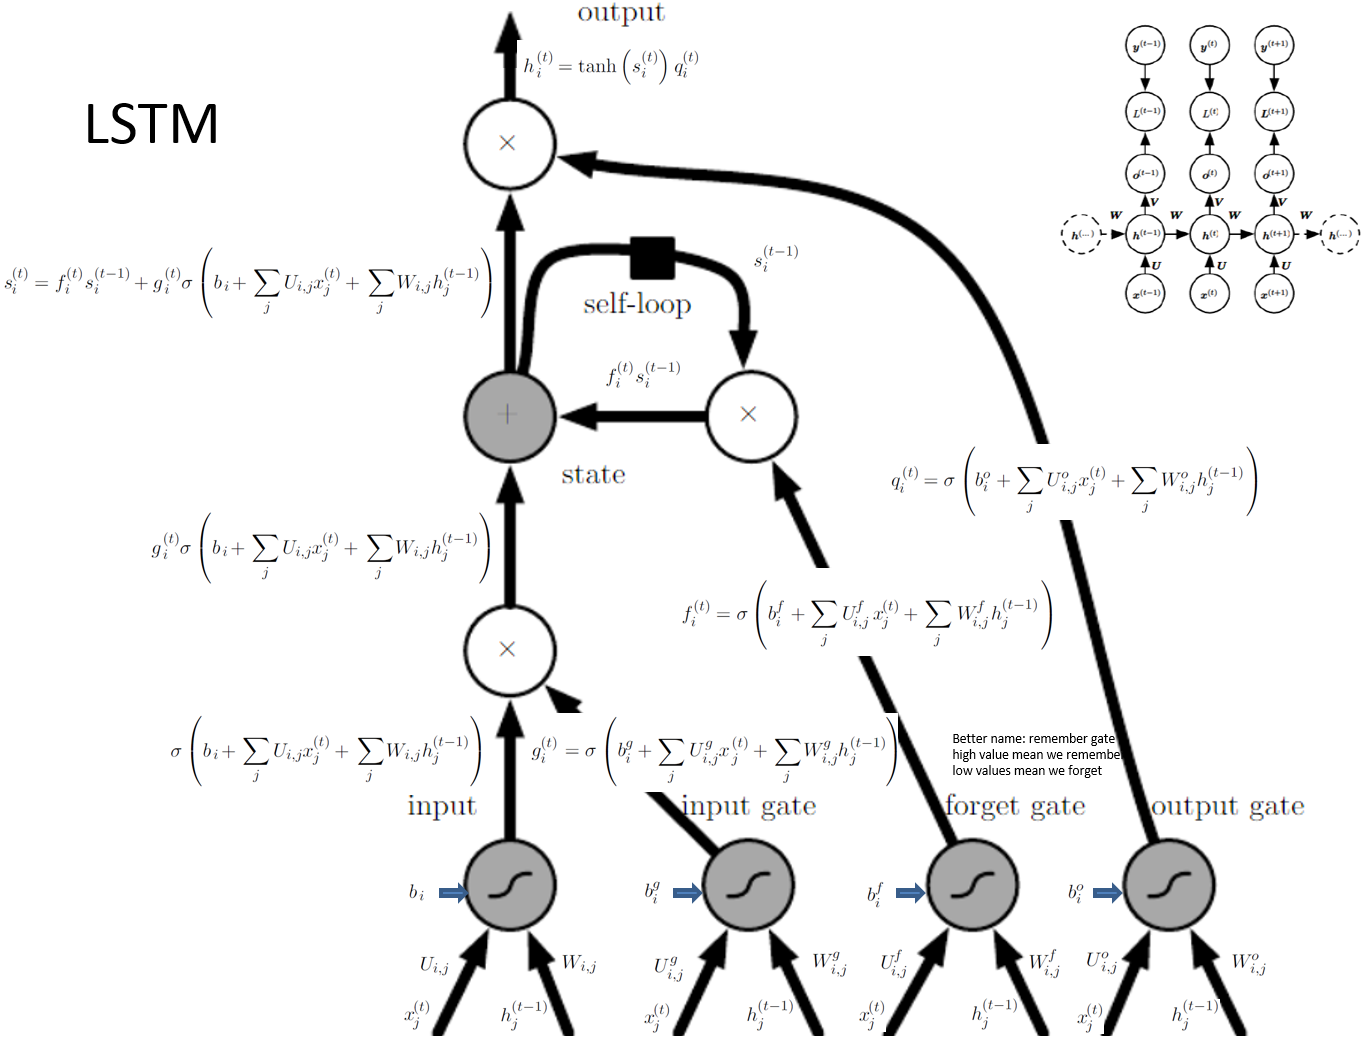
\includegraphics[width=\linewidth]{images/lstm.PNG}
\end{figure}
LSTM networks have been found extremely successful in many applications:
\begin{itemize}
	\item Unconstrained handwriting recognition
	\item Speech recognition
	\item Handwriting generation
	\item Machine translation
	\item Image captioning and parsing
\end{itemize}
\begin{figure}[H]
	\centering
	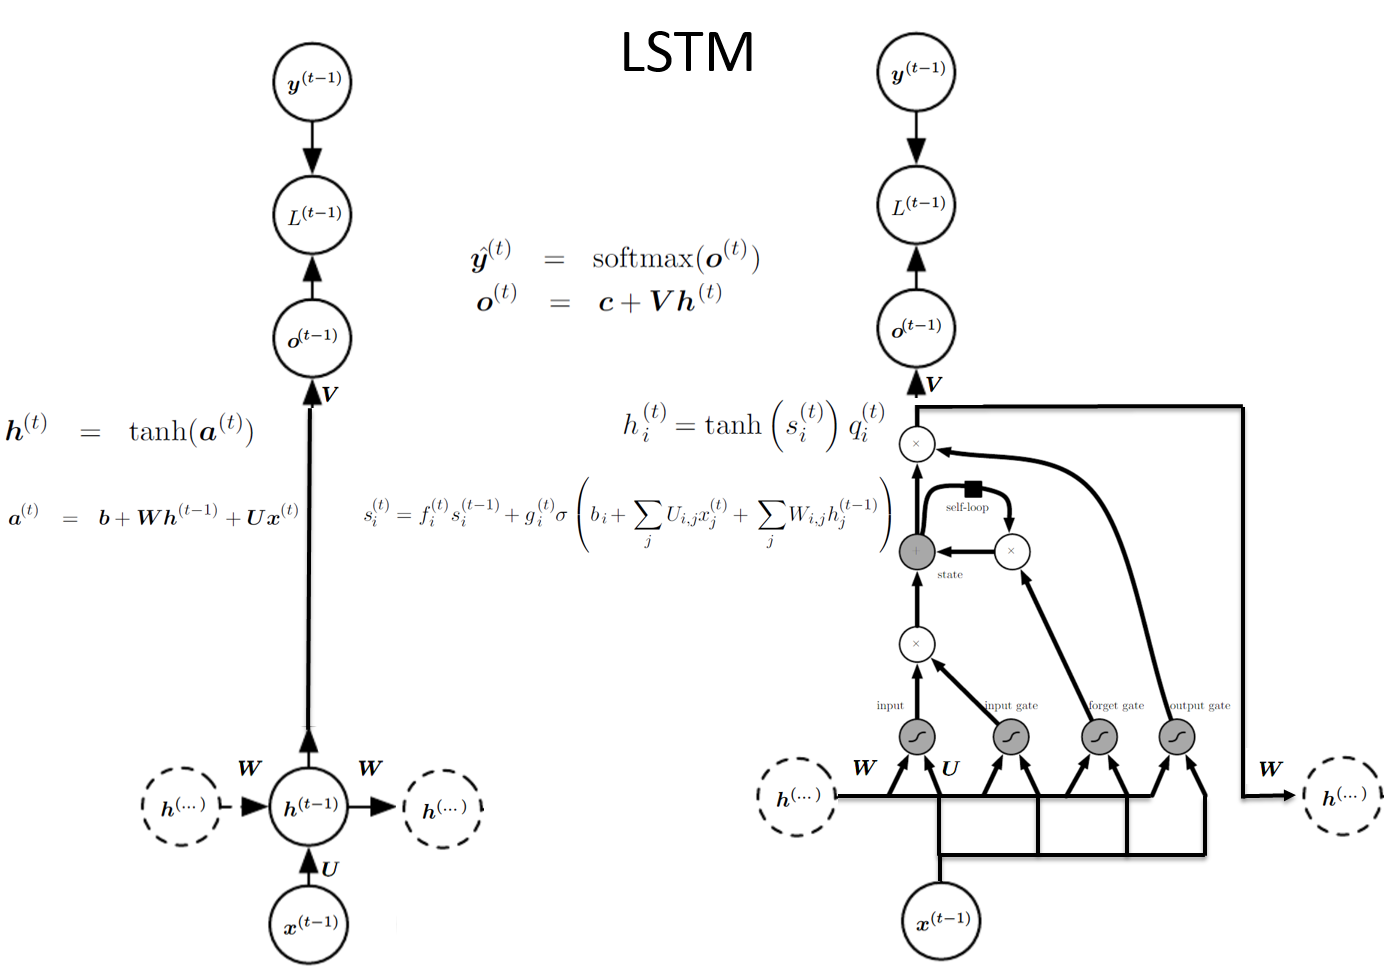
\includegraphics[width=0.9\linewidth]{images/lstm2.PNG}
\end{figure}
\begin{multicols}{2}
	\subsection{Other Gated RNNs}
	Which pieces of the LSTM architecture are necessary?
	Some answers to these questions are given by the work on gated RNNs, whose units are also known as gated recurrent units (\textbf{GRU}).
	The main difference with the LSTM is that a single gating unit simultaneously controls the forgetting factor and the decision to update the state unit.\\
	
	The update gates $u_i^{(t)}$ and reset gates $r_i^{(t)}$ can individually \emph{ignore} parts of the state vector.
	\begin{align*}
	u_i^{(t)} =& \sigma\left( b_i^u+\sum_j U_{i,j}^ux_j^{(t)}+\sum_j W_{i,j}^uh_j^{(t)} \right)\\
	r_i^{(t)} =& \sigma\left( b_i^r+\sum_j U_{i,j}^rx_j^{(t)}+\sum_j W_{i,j}^rh_j^{(t)} \right)\\
	h_i^{(t)} =& u_i^{(t-1)}h_i^{(t-1)} +(1-u_i^{(t-1)}) \\
	&\tanh \left( b_i+\sum_j U_{i,j}x_j^{(t-1)}+\sum_j W_{i,j}r_j^{(t-1)}h_j^{(t-1)} \right)\\
	\end{align*}
	\columnbreak
	The update gates act like conditional leaky integrators that can linearly gate any dimension, thus choosing to copy it (at one extreme of the sigmoid) or completely ignore it (at the other extreme) by replacing it by the new \emph{target state} value (towards which the leaky integrator wants to converge).
	The reset gates control which parts of the state get used to compute the next target state, introducing an additional nonlinear effect in the relationship between past state and future state.
	\begin{figure}[H]
		\centering
		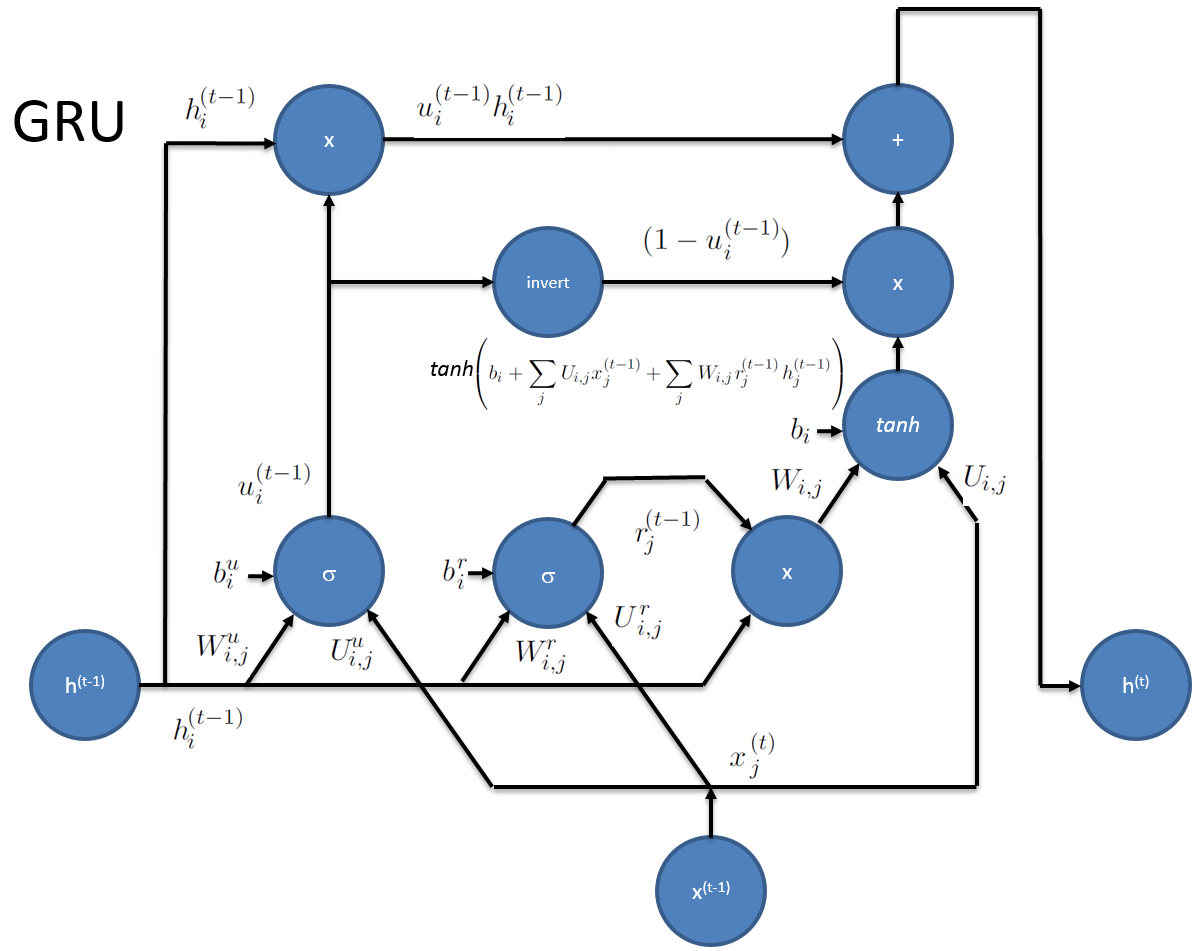
\includegraphics[width=1.05\linewidth]{images/gru.PNG}
	\end{figure}

\end{multicols}
\newpage




































